\documentclass[a4paper,11pt]{article}

\usepackage{xcolor}
\usepackage{relsize}
\usepackage{minted}
\usepackage[margin=2.25cm]{geometry}
\usepackage[hidelinks]{hyperref}
\usepackage{csquotes}
\usepackage[english, french]{babel} %last = main language

\MakeOuterQuote{"}
\usepackage[labelfont=bf, textfont=bf]{caption}
\usepackage[section]{placeins} %force figure in section
\usepackage{tabularx}
\usepackage{graphicx}
\usepackage{subcaption}
\usepackage{listings}
%caption setup
\DeclareCaptionFormat{myformat}{#1#2#3\hrulefill}
\captionsetup[subfigure]{format=myformat}

%traduction
% \renewcommand\listingscaption{Code}
\renewcommand\listoflistingscaption{Table des listings}

%force floats in section
\let\Oldsection\section
\renewcommand{\section}{\FloatBarrier\Oldsection}

\let\Oldsubsection\subsection
\renewcommand{\subsection}{\FloatBarrier\Oldsubsection}

\let\Oldsubsubsection\subsubsection
\renewcommand{\subsubsection}{\FloatBarrier\Oldsubsubsection}

%centered wrapping column
\newcolumntype{Y}{>{\centering\arraybackslash}X}

\title{BE Qualité de service dans l'internet \\[0.1em]\textsmaller[]{4IR SC - INSA Toulouse - DGEI}}
\author{
    \begin{tabular}{cc}
        Thomas Bobillot & Philippe Hérail \\
        \texttt{bobillot@etud.insa-toulouse.fr} &\texttt{herail@etud.insa-toulouse.fr} \\
        Léo Picou & Eva Soussi \\
        \texttt{picou@etud.insa-toulouse.fr} &\texttt{soussi@etud.insa-toulouse.fr}
    \end{tabular}
}

\begin{document}

\maketitle

\tableofcontents

\cleardoublepage

\section{Introduction}

Dans le cadre de l’UF "Interconnexion avancée de Réseaux", nous avons eu l’opportunité de réaliser ce bureau d’étude lié à la qualité de service. Il s’agissait de réaliser la mise en place, sur une journée, d’une solution de gestion statique de la QoS dans un réseau de coeur ainsi que d’une solution dynamique de la QoS sur un réseau client. Des séances de TP et de travail personnel nous ont permis de préparer ce travail en amont de la journée du 29 mai.

Ce rapport a pour but de présenter l’ensemble des choix réalisés pendant la préparation et pendant la journée de réalisation. Il présentera tant la stratégie d'implémentation que sa réalisation.

\section{Architecture}

\begin{figure}[htp]
    \centering
    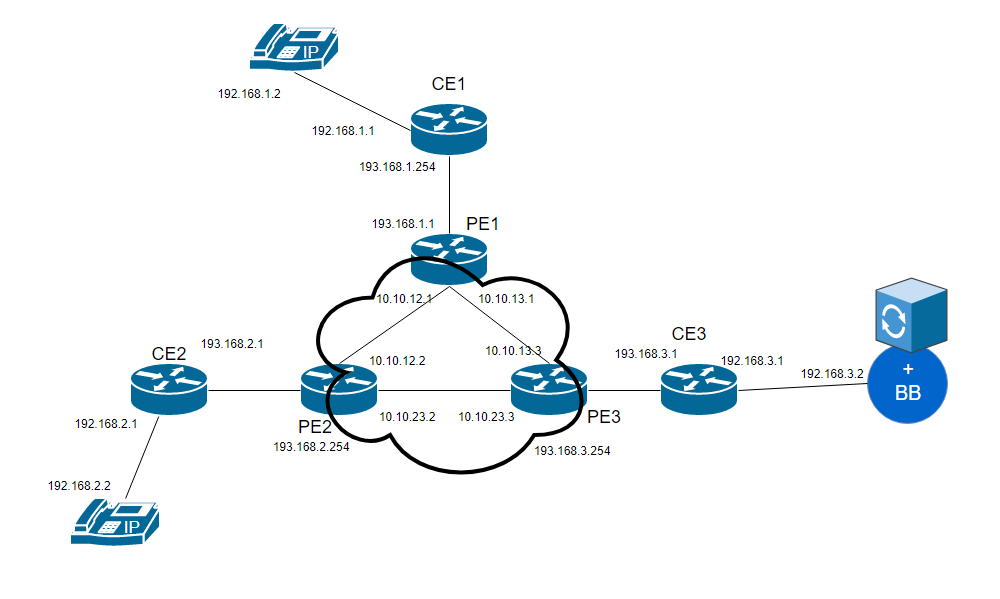
\includegraphics[width=\textwidth]{images/archrzo.png}
    \caption{Architecture du réseau}
    \label{fig:archrzo}
\end{figure}

L’architecture à mettre en place est celle présentée en Figure \ref{fig:archrzo}. Trois réseaux d’un même client sont interconnectés grâce au réseau de coeur. 
Pour jouer le rôle des routeurs de bordure du réseau de coeur (Provider Edge, PE), nous avons utilisé des routeurs Cisco. 
Les routeurs de bordures de réseaux clients (Customer Edge, CE) ont quant à eux été mis en place à l'aide de routeurs Linux. Deux sites étaient supposés héberger des softphones, tandis le troisième devait héberger le Bandwith Broker ainsi que le Proxy SIP. Les softphones n’ont pas fonctionné pour la journée QoS, et nous avons donc utilisé des téléphones Cisco à la place. 

\section{Réseau de coeur}

Nous avons mis en place un domaine IP/MPLS DiffServ. 
La première phase du déploiement a été de mettre en place le domaine IP/MPLS. Pour cela, nous avons suivi les étapes suivantes :
\begin{itemize}
    \item Activation d'OSPF, afin d’alimenter les tables de routage.
    \item Activation du protocole LDP.
    \item Activation de MPLS sur les interfaces réseau appartenant au domaine MPLS.
    \item Mise en place de l'architecture VPN-IP, via la configuration des VRF et leur association aux sites. Les VPN assurent l’isolation du trafic entre les sites clients, qui possèdent dans notre cas des adresses privées.
    \item Etablissement des sessions MP-BGP entre les PE, capable d'échanger des inforamtions de routage VPNv4.
\end{itemize}

Nous avions donc un réseau sécurisé via un VPN de niveau 3, car nous étions plus à l'aise avec la mise en place de type de VPN, tout en satisfaisant les contraintes imposées par le sujet du BE. 

Afin de pouvoir mettre en place de la qualité de service dans notre réseau, nous avons dans un second temps mis en place un domaine DiffServ sur ce réseau de coeur. 

Nous avons établi un SLA pour chaque client, donc pour chaque connection entre CE et PE. Celui-ci est identique pour chacun des sites, mais rien dans notre travail n'interdirait de créer des SLA différents. D’après ce SLA, on veut garantir 25\% de la capacité des liens série interconnectant nos routeurs du réseau de coeur pour la voix, soit 2 Mbit/s. 
La politique de policing suit le SLA et garantit que les clients ne dépassent pas le volume de trafic qui leur a été accordé. Dans le cadre du SLA on assure une garantie sur deux types de trafic : BE (best effort) et TR (temps réel, voix). 

Au niveau du PE nous avons donc décidé de mettre en place deux classes DiffServ. Néanmoins, ce choix est discutable, car nous aurions pu définir plus de classes sans que cela impacte le système, tant que nous respections globalement la capacité de nos liens. Nous aurions par exemple pu définir une troisième classe de trafic, pour prioriser les flux à l’intérieur du nuage MPLS concernant les protocoles de routage (par exemple pour les flux ospf, ldp, etc...) qui sont encore plus fortement prioritaire. Pour des questions de simplicité de mise en place, nous ne l’avons pas fait dans le cadre de cet exercice.

Pour notre cas, nous avons donc défini deux classes de trafic en fonction de la priorité, détaillées ci-après : 
\begin{description}
    \item[TR] pour le trafic en temps réel, et donc dans le cas de notre application la voix
    \item[BE] pour le trafic géré en best effort, pour les types de flux non prioritaires (tous les autres flux)
\end{description}

Nous avons ainsi mis en place des règles de policing sur ces classes de service. La plus grande limitation du réseau concerne les liens série. Pour respecter le SLA au niveau des 2 Mbit/s : on alloue un quart de la capacité du lien série à la voix soit. De plus, si on a un trafic plus grand que 2 Mbit/s en TR au niveau de l'entrée du PE, on élimine tout simplement les paquets non conformes. 

Au sein du nuage MPLS, le domaine DiffServ est mis en place en suivant les deux mêmes classes. La classification du trafic se fait en raisonnant sur le champ EXP de l’entête MPLS, dans lequel on recopie les 3 bits de poids fort du champs DSCP du paquet IP. Lorsque le paquet quitte le domaine MPLS, le champ EXP du dernier entête MPLS est recopié dans le champ DSCP, afin de permettre une continuité


\section{Bandwidth Broker}
\label{sec:BB}
Le Bandwidth broker a été écrit en Java. Ce langage a été choisi pour la facilté de déploiement de logiciel en salle de TP, mais également suite au travail effectué dans ce langage au premier semestre. Ceci a permis de réutiliser les connaissances acquises, principalement au niveau de la communication en réseau.

Le Bandwidth Broker (BB) est articulé autour des classes présentées ci-après et détaillées dans les section suivantes.

\begin{description}
    \item[\texttt{Main}] point d'entrée de l'application, ainqi qu'une fonction d'écoute et de communication avec le proxy SIP.
    \item[\texttt{BandwidthBroker}] présente les fonctions attendues du BB : enregistrement de nouveaux sites, que l'ajout et le retrait de réservations de bande passante et l'envoi des commandes de configuration du routeur.
    \item[\texttt{Site}] implémente, site par site, la réservation de bande passante, et le stockage des informations liées à un site, telles que le netmask, les adresses des interfaces du routeur de bordure, et les informations du SLA, et la génération des commandes de configuration des routeurs de bordure.
    \item[\texttt{ReservationData}] contient les informations nécessaires à la réservation, à savoir le couple source\slash destination et la bande passante nécessaire. Permet d'abstraire les échanges SIP au niveau du reste de l'application.
\end{description}

Cette application communique avec le proxy SIP via un socket TCP, via l'envoi de classes sérialisées, et le BB communique avec les différents routeurs de bordure grâce à un socket TCP qui envoie les commandes de manières textuelles, via un simple socket, à une instance de \texttt{netcat} executant toutes les commandes reçues. 
Les classes sérialisées nous permettent d'échanger facilement des informations arbitraires entre le proxy et le BB, via le simple partage du code de deux classes \texttt{QoSRequest} et \texttt{QoSResponse}, ce qui permet d'éviter l'utilisation de bibliothèques externes, pouvant poser des difficultés de déploiement.
L'instance \texttt{netcat}, utilisée avec l'option \texttt{-e /bin/bash} et les droits root permet de simplifier la mise en place de la communication entre le BB et les routeurs CE, à comparer de la solution que nous avions envisagée reposant sur l'établissement d'une session SSH, nécessitant alors la mise en place de clés de chiffrement.

De plus, différentes classes ont été créés dans le package \texttt{utils}, visant à centraliser certaines fonction utilitaires, telles que la conversion d'une adresse IP sous forme de \texttt{String} vers un \texttt{Integer}, afin de permettre des opérations bit à bit sur  celle-ci. Ces fonctions étaient disponibles dans des bibliothèques Apache, cependant leur simplicité à mettre en oeuvre permettait d'éviter des difficultés possibles lors du déploiement de bibliothèques supplémentaires.


\subsection{Class \texttt{Main}}

Cette classe permet de configurer les différents site, via l'appel à une fonction du BB (voir Listing \ref{lst:confsite}). Afin de se concentrer sur l'implémentation des fonctions spécifiques au BE, les différents sites sont configurés dans le code même.

\begin{listing}[htp]
    \begin{minted}[frame=single,framesep=10pt]{java}
Site site1 = new Site(netmask,
                    ipStringToInteger("192.168.1.1"), //IP interne routeur
                    "eth1", //interface interne routeur
                    ipStringToInteger("193.168.1.1"), //IP externe routeur
                    "eth0", //interface externe routeur
                    4444, //port d'écoute netcat
                    2000); //capacité EF, en kbits
BB.addSite(site1, 1);
  \end{minted}
    \caption{Configuration d'un site}
    \label{lst:confsite}
\end{listing}

La fonction de communication avec le proxy SIP est également implémentée directement dans la fonction main, en raison de la simplicité de celle-ci. En effet, nous avons choisi de travailler avec une application monothreadée,  afin de simplifier son développement, ce qui a été suffisant de le cadre du projet, en raison du peu de requêtes reçues de la part du proxy SIP.

\subsection{Class \texttt{BandwidthBroker}}

La classe contient 3 structures de données (Listing \ref{lst:stockagesite}). Les deux premières structures permettent d'accèder à un site à la fois par son index, et par l'adresse de réseau interne. Les index permettent de simplifier la configuration de sites  à l'aide boucles \texttt{foreach}, mais également d'établir une correspondance évidente avec les numéros de site du BE.
L'accès par réseau permet d'identifier un site depuis les informations obtenues grâce aux requêtes du proxy SIP.

La dernière structure, \texttt{socketIndexer}, est principalement liée à l'utilisation de \texttt{netcat}. En effet, puisque la session est fermée lors de la déconnexion, il est nécessaire de conserver celle-ci ouverte, et donc de conserver ouvert le socket. 
Nous avons fait le choix de créer la connection lors de l'ajout du site au BB, et non lors de la création de l'objet \texttt{Site}. \texttt{SocketIndexer} nous permet ainsi de garder une référence vers le socket pour l'ensemble de la durée de de vie de l'instance du \texttt{BandwidthBroker}, et d'y accèder via l'index du site afin d'envoyer les commandes de configuration nécessaires.


\begin{listing}[htp]
    \begin{minted}[frame=single,framesep=10pt]{java}
// Stores the associations network/SiteIndex
Map<Integer, Integer> networkIndexer;

// Stores the couples SiteIndex/Site
Map<Integer, Site> siteIndexer;

// Stores couples SiteIndex/Socket
Map<Integer, Socket> socketIndexer;
      \end{minted}
    \caption{Stockage des différents sites}
    \label{lst:stockagesite}
\end{listing}

Lors de l'ajout d'un site au BB, celui-ci va directement envoyer une série de commandes permettant de réinitialiser la configuration du shaping, en créant la file parent nécessaire pour la voix, ainsi que la table \texttt{mangle} de \texttt{iptables}.


\subsection{Class \texttt{Site}}

Cette classe permet de stocker les différentes informations sur l'état d'un site, détailllées dans le Listing \ref{lst:infosite}.
Il implémente également les méthodes permettant de connaitre la possibilité d'effectuer une réservation, mais également de l'effectuer le cas échéant, et de la  supprimer sur demande du BB.
L'attribut \texttt{queueReservationList} permet de retrouver l'index de la file à détruire lors d'une requête de dé-réservation du proxy SIP.

\begin{listing}[htp]
    \begin{minted}[frame=single,framesep=10pt]{java}
private Integer netmask; //Netmask associé au réseau interne du site
private Integer edgeRouterIPinside;
private String edgeRouterInterfaceInside;
private Integer edgeRouterIPoutisde;
private String edgeRouterInterfaceOutside;
private Integer netcatPort;
private Integer totalEFCapacity; //Capacité de trafic temps réel du site
private Integer usedEfCapacity; //Capacité de trafic temps réel utilisée 
private Map<ReservationData, Integer> queueReservationList;
private Integer tcqueueIndexCounter; //Compteur des index de listes, 
                                     //permet d'identifier les files créées
    \end{minted}
    \caption{Informations stockées par une instance de \texttt{Site}}
    \label{lst:infosite}
\end{listing}

Cette classe permet aussi de générer les commandes de configuration de \texttt{tc} et \texttt{iptables}, donc un exemple est donné dans le Listing \ref{lst:genconfig}. Ces commandes sont ensuite envoyées par le BB à lors de la procédure de réservation de bande passante.

\begin{listing}[htp]
    \begin{minted}[frame=single,framesep=10pt]{java}
private String generateConfigStringTc(Integer dataRateReq) {
        String s = "tc class add dev " + this.getEdgeRouterInterfaceOutside() 
        + " parent 1:1 classid 1:1"
        + this.getTcqueueIndexCounter() + " htb rate " 
        + dataRateReq/1000 + "kbit ceil " 
        + dataRateReq/1000 + "kbit";
        return s;
    }

    \end{minted}
    \caption{Exemple de génération des commandes de configuration du routeur}
    \label{lst:genconfig}
\end{listing}

\subsection{Class \texttt{ReservationData}}

La classe \texttt{ReservationData} permet de stocker, comme expliquée précédemment, les couples \NoAutoSpacing{SourceIP:Port\slash DestinationIP:Port}, ainsi que la bande passante nécessaire pour la communication associée.

Cependant, il est important de noter que cette classe remplace les méthodes \texttt{equals()} et \texttt{hashCode()} afin de permettre de comparer deux réservation seulement à partir de la source et de la destination, comme par exemple dans le \texttt{tcqueueIndexCounter} de la classe \texttt{Site}.


\section{Traffic control}

\begin{figure}[htp]
    \centering
    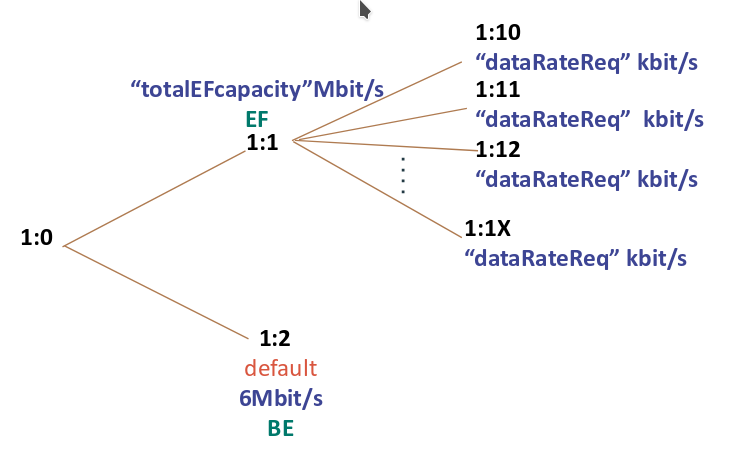
\includegraphics[width=\textwidth]{images/tc.png}
    \caption{Files HTB configurées par le BB}
    \label{fig:htb-files}
\end{figure}

La Figure \ref{fig:htb-files} représente les files Hierarchical Token Bucket (HTB) qui ont été mises en place pour assurer le \emph{traffic shaping} des CE. 
A l’initialisation du CE par le BB sont mises en places les files 1:0 (file racine), 1:1 (traffic temps réel) et 1:2 (file par défaut)). La file 1:2 vise à recevoir tout le trafic de type Best Effort. En parallèle, on a renseigné une règle \texttt{iptables} orientant tout le trafic dans la file 1:2 en l'absence d'autres règles.

A chaque nouvelle demande de réservation, on crée une nouvelle file fille de 1:1 avec un débit max et garanti de “dataRateReq” kbit/s. Ce paramètre est un attribut de la classe \texttt{ReservationData} du BB et est présent pour permettre une allocation de bande passante différente selon le codec utilisé pour la communication. On ajoute aussi à chaque nouvelle demande de réservation une règle \texttt{iptables} en tête de la table pour associer le trafic, destiné à l’adresse IP destinataire et au port spécifique à la communication, à la file fraîchement créée. 

Quand une communication est terminée, on retire l’ensemble des règles associées à cette communication (les filtres \texttt{tc} ainsi que les règles de \texttt{iptables}) et on finit par supprimer la file HTB.

La creation et la destruction des files est des règles associées sont automatisées par le BB, dont le fonctionnement a été détaillé en Section \ref{sec:BB}.

\section{Proxy SIP}

Les deux diagrammes de séquence du processus de réservation de bande passante par le proxy SIP sont présentés Figure \ref{fig:reqres}.

\begin{figure}[htp]
    \centering
    \begin{subfigure}{0.8\textwidth}
        \centering
        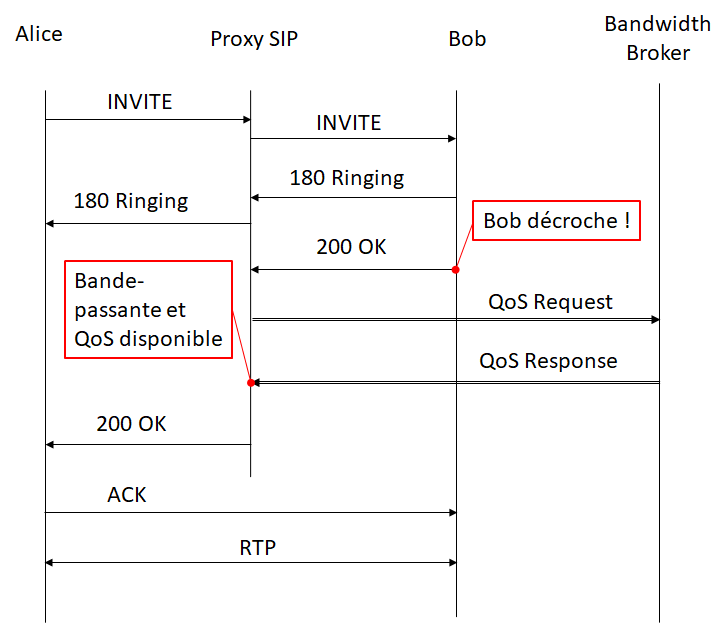
\includegraphics[width=\linewidth]{images/reqOK.png}
        \caption{Succès de la réservation}
    \end{subfigure}
    \begin{subfigure}{0.8\textwidth}
        \centering
        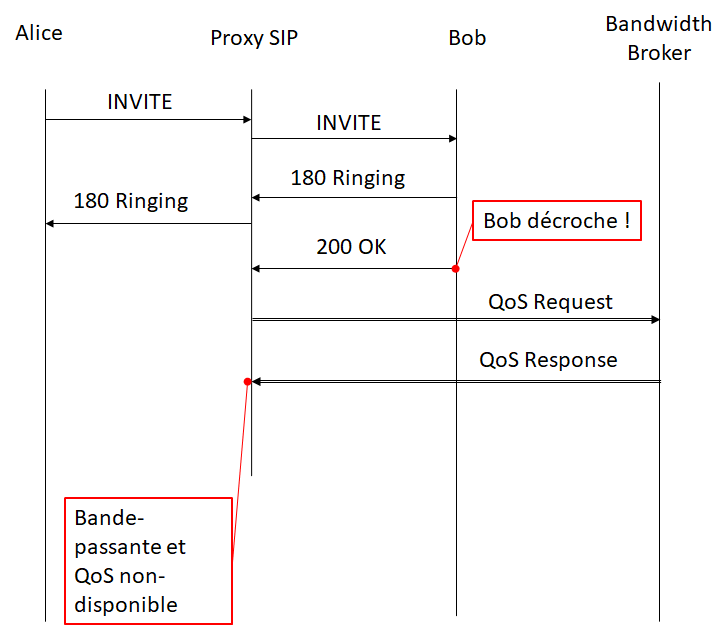
\includegraphics[width=\linewidth]{images/reqNOK.png}
        \caption{Echec de la réservation}
    \end{subfigure}
    \caption{Diagrammes de séquence du processus de réservation de bande passante.}
    \label{fig:reqres}
\end{figure}


Tout le protocole de forwarding des requêtes SIP est déjà géré par le programme présent. Il a fallu rajouter seulement 2 fonctionnalités :
\begin{itemize}
    \item Demande de QoS
    \item Traitement de la réponse QoS
\end{itemize}


Pour ce faire, nous avons modifié le code Java de la classe \texttt{Proxy} du package \texttt{openjsip.proxy}. 
Pour savoir précisément quand effectuer la requête de QoS, nous avons analysé en détail le protocole SIP. Il ne faut pas faire la requête de QoS avant que le destinataire (Bob) décroche, sinon des ressources peuvent être inutilement réservées dans le cas où le destinataire n’est pas disponible. Il ne faut pas non plus la faire trop tard sinon la communication pourrait être interrompue.
Pour en savoir davantage sur les paquets SIP reçus, nous avons modifié la méthode \texttt{processResponseStatelessly(...)} afin d’afficher en détail l’ensemble des entêtes. Grâce à ces informations et à la documentation disponible sur ce protocole, nous avons pu comprendre que la demande de QoS devait être effectué lorsque nous recevions un paquet avec un status code 200 OK sur une méthode INVITE. Ce paquet est envoyé par le téléphone destinataire lorsque Bob décroche. Ainsi, avant de forward ce paquet au téléphone de l'appelant (Alice) nous devons demander au Bandwidth Broker de réserver les ressources nécessaires. Nous avons par conséquent implémenté :

\begin{itemize}
    \item Une méthode \texttt{RequestToBB(...)} bloquante
    \item Un objet \texttt{QoSRequest}
    \item Un objet \texttt{QoSResponse}
\end{itemize}




Lorsque la situation décrite précédemment (200 OK \& INVITE) est rencontrée, nous créons un objet \texttt{QoSRequest} contenant l’ensemble des paramètres requis par le BB pour réserver les ressources nécessaires. 
Cette objet contient actuellement 3 informations :
\begin{itemize}
    \item L’adresse IP d’Alice
    \item L’adresse IP de Bob
    \item Le débit nécessaire
\end{itemize}




Pour obtenir les adresses IP, nous nous basons sur 2 champs du Header, \emph{From}  et \emph{To}. Pour connaître le débit nécessaire, nous nous basons sur le codec choisi dans le champ \emph{Media} du Header de la payload SDP. Une fois ces informations réunies, l’objet QoSRequest est envoyé au BB via \texttt{RequestToBB(...)}. Cette méthode retourne un objet \texttt{QoSResponse} contenant la réponse du BB. Cette réponse est modélisée sous forme d’un booléen :

\begin{itemize}
    \item True pour "Ressources disponibles, réservation effectuée !"
    \item False pour "Ressources indisponibles, réservation non-effectuée !"
\end{itemize}


En fonction de la valeur de ce booléen, on forward ou non le paquet SIP 200 OK \& INVITE à Alice.

On constate sur Wireshark que de nombreuses réémission de paquets surviennent. Le proxy SIP peut donc potentiellement recevoir plusieurs fois le paquet 200 OK \& INVITE, et réserver plusieurs fois la même bande-passante. Pour éviter cette situation, on vérifie aussi le champ \emph{Call-ID} dans l'entête SIP, qui est unique par appel. Pour chaque réservation effectuée, on ajoute le Call-ID correspondant dans une liste statique. Avant de faire une réservation, on vérifie si le Call-ID est déjà présent dans cette liste, si c’est le cas alors cela veut dire que c’est un paquet ré-émis, et que par conséquent la demande de réservation est inutile (puisque déjà effectuée).    

Pour l’instant seule l’adresse IP est utilisée pour effectuer la réservation, donc si l’on considère un softphone, l’utilisateur pourra malheureusement profiter de son appel en cours pour avoir des QoS avantageuse sur le reste de son trafic (surf web, téléchargement, etc...). Pour éviter cette situation, il faut préciser les ports RTP source et destinataire. Malheureusement le port source se trouve dans le paquet 200 OK \& INVITE émis par Bob, mais le port destinataire se trouve dans un paquet différent. Cela implique donc de modifier le code pour pouvoir mémoriser les anciens paquets.

Finalement, la libération des ressources pourrait être implémenté lorsqu’un utilisateur raccroche, et qu’un paquet avec la méthode BYE est envoyé. Malheureusement, sur toutes les traces wireshark relevées, aucune ne contenait de paquet BYE. Nous pensons que les téléphones Cisco utilisés en TP n'implémentent pas cette partie du protocole SIP, par conséquent nous ne pouvons pas libérer les ressources. Cela nuit très gravement au réseau et rends le projet relativement inutile. Nous pourrions tout de même tenter d’implémenter une libération de ressource en plaçant des sniffeurs aux endroits stratégique du réseau, qui pourraient assez facilement détecter qu’un flux RTP s’interrompt dans les deux sens (Alice raccroche, et Bob aussi). Lors de cette détection, ces sniffers enverraient au BB une demande de libération pour signifier que l’appel est terminé. Tout cela sort cependant du cadre du BE. 


% \section{Réalisation} 

% La transmission au sein du réseau de coeur est assurée de manière efficace. Lorsqu’on sature le lien série, les 2 Mbit/s pour la voix sont garantis, et le trafic best effort peut uniquement profiter des 6Mbits restants. Des débits un peu plus bas peuvent être acceptés étant donné toute la payload induite (par les vrf, labels mpls, encapsulation VPN) ainsi que tout le trafic ospf, mp-bgp etc qui circule en permanence dans le réseau de cœur utilise une partie de la bande passante disponible.

% Concernantl le policing, on a remarqué que les débits lorsque nous dépassions les 2 Mbit/s de traffic voix, le débit obtenu était bien plus faible qu'atendu, aux environs de 1,6 Mbit/s. 
% Après différents tests, nous nous sommes rendus compte que ceci était causé par la fragmentation. En évitant cette fragmentation, nous arrivons 

\section{Conclusion}

En conclusion, ce projet nous aura permis de consolider nos compétences en réseau ainsi qu’en programmation orientée objet en Java. 

Ce bureau d'étude nous a également offert l’opportunité d’expérimenter un mode de travail différent de celui habituellement mis en place à l’INSA : la journée entière était dédiée au même sujet, nous étions donc invités à y concentrer toute notre attention et mobiliser toutes nos connaissances pour son aboutissement.
Bien que stressés au début, nous avons aussi avec le recul apprécié son format singulier : une journée pour atteindre les objectifs prévus (ou tout du moins s’en approcher au mieux), avec la nécessité de composer avec les imprévus. 

Ces deux points étaient des singularités dans le paysage du format d’études que nous effectuons, mais nous ont pour sûr été bénéfiques, puisqu’ils nous ont permis de mettre un premier pied dans la réalité du monde professionnel de l’ingénieur. 


\cleardoublepage
\listoflistings
\listoffigures

\end{document}